\section{Iteración 4}

Para darle una mayor accesibilidad al sistema se decidió desarrollar
una aplicación web, de este modo cualquier persona con conexión a
Internet podría acceder a ella. El siguiente paso en el desarrollo
del proyecto sería darle acceso a cualquier persona con internet.

Para ello tendrá que estar alojada en algún servidor externo.
Puesto que no guardamos ningún dato sensible, no hace falta
que esté alojado en Europa. Después de analizar las distintas posibilidades
se decide usar Heroku. Para ello se hizo un estudio de las herramientas
de hosting mas conocidas cuyo resultado se puede ver en la \hyperref[tab:Tabla comparativa precios hosting]{tabla 5.7}

\begin{longtable}{|p{0.1\linewidth}p{0.1\linewidth}p{0.1\linewidth}p{0.1\linewidth}p{0.15\linewidth}p{0.15\linewidth}p{0.15\linewidth}|}
  \caption{Tabla comparativa precios hosting}
  \label{tab:Tabla comparativa precios hosting}
  \endfirsthead
  \endhead
  \hline
  \multicolumn{1}{|l}{Hosting} & Precio & Dominio incluido & Soporte incluido & Documentación & Retraso en primer acceso & Nº máximo de instancias \\ \hline
  Heroku & 0€ & No & No & Media & 30 segundos & 5 \\ \hline
  AWS & 0.69€ & No & Si & Alta & 0 segundos & 1 \\ \hline
  Azure & 0.49€ & No & Si & Alta & 0 segundos & 1 \\ \hline
  IBM Cloud & 0€ & No & No & Media & 30 segundos & 1 \\ \hline
\end{longtable}

Para mejorar el desarrollo del proyecto aplicó integración continua gracias
a la creación de test, comprobación de cobertura de código en test y además
calidad de código usando rubocop. Para ello se utilizó CircleCI el cuál te
permite crear un conjunto de trabajos los cuales deberán tener una salida
positiva o negativa en función de si han sido satisfactorios o no sus resultados.

Primero se descargará la máquina e instalarán las dependencias necesarias.
Esto se hace para comprobar que no hay conflictos entre ellas y que todas
están disponibles. Después se crea la base de datos con todas las migraciones
necesarias. De este modo comprobamos que no hay problemas a la hora
de generar una base de datos y no habrá problemas en el despliegue.
Con la base de datos creada se lanzan todo el conjunto de test al completo.
En caso de que falle alguno este trabajo no será satisfactorio y el CI
fallará. Cuando se hayan pasado todos los test entonces se ejecutará
una tarea para comprobar que la calidad de código es correcta.

Estos trabajos se comprueban con cada subida al repositorio, ya sea una rama
diferente de la principal o la misma. En la \hyperref[fig:Ejemplo pull request]{figura 5.11}
se puede ver un ejemplo de una pull request de una rama secundaria en la que
fallaron estos trabajos pero al final todos fueron positivos.

\begin{figure}[htb]
  \centering
  \scalebox{.8}{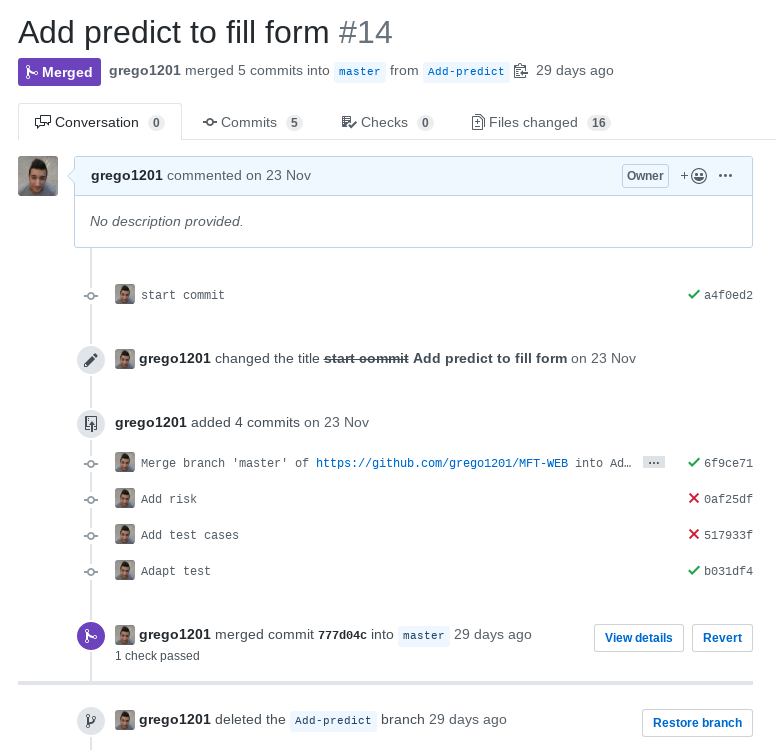
\includegraphics[width=0.8\linewidth]{CI}}
  \caption[Ejemplo pull request]{Ejemplo pull request}
  \label{fig:Ejemplo pull request}
\end{figure}

Gracias a estos trabajos se puede tener integración continua. Heroku facilita
esta labor con sus integraciones de GitHub. Una vez conectamos las cuentas se
puede elegir el despliegue manual o el automático, seleccionando una rama principal.
En este proyecto la rama principal será master. Cuando se haga una subida a master
se lanzarán todos los trabajos que comprueban que todo está correcto y una vez hayan
pasado todos se subirán los cambios automáticamente a la página web y se verán reflejados.
De esta manera se ahorra mucho tiempo de trabajo evitando despliegues manuales, llevando estos
a posibles errores como subir cosas que no se deba u olvidar algún paso en el proceso
de despliegue.
